\documentclass[xcolor=pdftex, dvipsnames, table]{beamer}

\RequirePackage[russian]{babel}
\RequirePackage[utf8]{inputenc}
\RequirePackage[TS1,T2A]{fontenc}
\usepackage{float}
\usepackage{amsmath}
\usepackage{listings}

\floatstyle{ruled}
\newfloat{program}{h}{src}
\floatname{program}{Листинг}

\usepackage{beamerthemeBoadilla}

\title{Система учёта и управления электронными налоговыми декларациями.}
\author{Залунин Павел}
\institute {
  БГУИР\\
  ФИТУ
}

\begin{document}

\frame{\titlepage}

\section[Outline]{}
\frame{\tableofcontents}

\section{Введение}
\subsection{Актуальность}
\begin{frame}
  \frametitle{Актуальность}
  \begin{block}{Проблемма}
    Заполнение финансовых документов весьма трудоемкий процесс, включающий в себя операции с большим объемом данных. Данные представляют собой различные аспекты деятельности предприятия, которые так же необходимо учитывать. Правила заполнения финансовых документов меняются как минимум раз в финансовый год. На больших предприятиях существует потребность в заполнении большого количества документов, что влечет за собой большие финансовые затраты.
  \end{block}
\end{frame}

\subsection{Налоговая декларация}
\begin{frame}
  \frametitle{Налоговая декларация}
  \begin{block}{Налоговая декларация}
    Налоговая декларация - документ, содержащий данные о финансовой деятельности предприятия.


Существуют различные налоговые формы ( активные доходы, пассивные доходы, налог на $CO^{2}$ и др.)
  \end{block}
  \begin{center}
    \includegraphics[width=0.9\textwidth,maxheigth=0.9\textheight]{pics/declaration}
  \end{center}
\end{frame}

\begin{frame}
  \frametitle{Существующие решения}
  Были рассмотрены следующие коммерческие решения:
  \begin{center}
    \small {
      \rowcolors{1}{RoyalBlue!20}{RolalBlue!5}
      \begin{tabular}{|p{2cm}|p{2cm}|p{1.5cm}|p{1.6cm}|p{2.3cm}|}\hline
        \bfseries{Название системы} &
        \bfseries{Тип} &
        \bfseries{ОС} &
        \bfseries{Структура} &
        \bfseries{База Данных}\\
        \hline
        1C Бухгалтерия & Система бухгалтерского учета & Windows, GNU Linux & Standalone, Web & 1CD, Microsoft SQL Server, DBF\\
        \hline
        Галлактика ERP & СПРП\footnote[1]{Система планирования ресурсов предприятия\label{erp}} & Windows  & Standalone  & PervasiveSQL, Microsoft SQL Server, Oracle\\
        \hline
        Парус & СПРП$^{1}$ & Windows & Standalone, Web & Oracle\\
        \hline
        Microsoft Dynamic NAV & СПРП$^{1}$ & Windows & Standalone, Web & Microsoft SQL Server\\
        \hline
      \end{tabular}
    }
  \end{center}
  \\
\end{frame}


\section{Проектирование}
\subsection{Структура системы}
\begin{frame}
  \frametitle{Структура системы}
  \begin{center}
    \includegraphics[width=0.7\textwidth,maxheight=0.8\textheight]{pics/system_struct}
  \end{center}
\end{frame}
\subsection{Требования}
\begin{frame}
  \frametitle{Требования, предъявленные к системе}
  \begin{itemize}
    \item Web интерфейс;
    \item использование реляционной БД;
    \item возможность добавление новых деклараций и изменения существующих, необходимо предоставить простой способ для достижения этой цели;
    \itemредактирование декларации должно осуществляться интерактивно, без перезагрузки страницы;
    \itemподдержка трех типов ячеек: a) формула b) интервальная c) пользовательская;
    \itemтребуется предоставить возможность задания произвольного значения для ячейки, которая считается по каким-либо правилам.
  \end{itemize}
\end{frame}

\begin{frame}
  \frametitle{Проектирование системы}
  \begin{itemize}
    \item Выделение объектов: диаграмма сущность связь
    \item Выделение вариантов использования: диаграммы вариантов использования
    \item Анализ вариантов использования: диаграммы последовательности
    \item Детализация объектов: выделение новых объектов, алгоримты подсчёта ячеек, грамматика языка для описание формул, диаграмма активности
    \item Представление структуры декларации на языке XML
    \item Логическая модель базы данных
  \end{itemize}
\end{frame}

\subsection{Типы ячеек}
\begin{frame}
 \frametitle{Ячейка типа <<Счета>>}
  \begin{columns}
    \begin{column}{0.4\textwidth}
      \begin{block}{Правило подсчета}
        Параметрами данной ячейки являются <<Интервалы>>, содержащие параметры: a) начало интервала b) конец интервала c) знак (+, -) d) тип (дебет, кредит). Значение считается как сумма дебетов либо кредитов <<Счетов>> из бухгалтерской книги, попавших в интервалы, с определенным знаком.
      \end{block}
    \end{column}
    \begin{column}{0.6\textwidth}
      \begin{figure}
        \includegraphics[width=0.65\textwidth]{pics/algo_accounts_calc}
        \caption{Алгоритм подсчета ячейки типа <<Счета>>}
      \end{figure}
    \end{column}
  \end{columns}
\end{frame}
\begin{frame}
  \frametitle{Ячейка типа <<Формула>>}
  \begin{columns}
    \begin{column}{0.5\textwidth}
      \begin{block}{Правило подсчета}
        Значение данной ячейки вычисляется по формуле. Примеры формул:
        \begin{itemize}
          \item \{A1\}+\{A2\}*\{A3\}
          \item ROUND(\{A1\})+\{A2\})
          \item MAX(\{A1\},\{A2\},\{A3\}) + MIN(\{A7\},\{A8\})
          \item SUM(A000,A999) + \{A2\}
        \end{itemize}
      \end{block}
    \end{column}
    \begin{column}{0.5\textwidth}
      \begin{figure}
        \includegraphics[width=0.65\textwidth]{pics/eval_algorithm}
        \caption{Алгоритм вычисления значения выражения}
      \end{figure}
    \end{column}
  \end{columns}
\end{frame}
\begin{frame}[fragile]
  \begin{block}{Грамматика (расширенная форма Бэкуса-Наура)}
    \begin{verbatim}
      number = integer | double
      simple_expr = number | str_const | variable
                   | func_call | '(',expression,')'
      unary_op = '-' | '!'
      bin_op = '<' | '>' | '<=' | '>='
             | '+' | "-" | '*' | '/' | '&'
             | '&&' | '||' | '^'
      expression = simple_expr | unary_op expression
             | {bin_op, expression }
      func_call = ident, '(',  ')' | ident, '(', params, ')'
      params = expression | expression ',' params
    \end{verbatim}
  \end{block}
\end{frame}

\section{Реализация}
\subsection{Инструментальные средства разработки}
\begin{frame}
  \frametitle{Процесс реализации системы}
  \begin{enumerate}
    \item Выбор инструментальных средств разработки
    \item Реализация классов-сущностей
    \item Реализация подсистемы управления
    \item Реализация подсистемы управления декларацией
    \item Реализация подсистемы хранения
    \item Реализация подсистемы отображения
    \item Реализация подсистемы вычисления значения выражения
    \item Тестирование системы
  \end{enumerate}
\end{frame}
\begin{frame}
  \frametitle{Инструментальные средства}
  \begin{itemize}
    \item Язык программирования Java.
    \item Набор библиотек Spring (использовались модули Spring MVC, Spring IoC).
    \item Библиотека Hibernate. Для реализации подсистемы хранения.
    \item Среда разработки Eclipse.
    \item Библиотека JUnit. Для тестирования.
    \item Сервер приложений Apache Tomcat. Для развертывания приложения.
    \item Технология Java Server Pages. Для реализации страниц.
    \item Язык сценариев JavaScript. Для реализации динамических страниц.
    \item Технология AJAX. Для работы с асинхронными запросами.
    \item Средство сборки приложений Maven.
  \end{itemize}
\end{frame}

\subsection{Реализация компонентов системы}
\begin{frame}
  \frametitle{Подсистема управления}
  \begin{columns}
    \begin{column}{0.6\textwidth}
      \begin{center}
        \begin{figure}
          \includegraphics[scale=0.23]{pics/springmvc}
          \caption{Обработка запроса Spring MVC}
          \label{pic:springmvc}
        \end{figure}
      \end{center}
    \end{column}
    \begin{column}{0.5\textwidth}
      Были реализованы следующие контроллеры:\\
      \begin{itemize}
        \item CompanyController
        \item TaxKitController
        \item TaxKitEditController
        \item LedgerController
        \item ReportStateController
        \item ReportController
      \end{itemize}
    \end{column}
  \end{columns}
\end{frame}

\begin{frame}
  \frametitle{Подсистема хранения}
  Объектно-реляционное отображение. Библиотека Hibernate.
  \begin{center}
    \includegraphics[width=0.9\textwidth]{pics/orm}
  \end{center}
\end{frame}

\begin{frame}
  \frametitle{Интерфейс пользователя. Редактирование декларации.}
  \begin{center}
    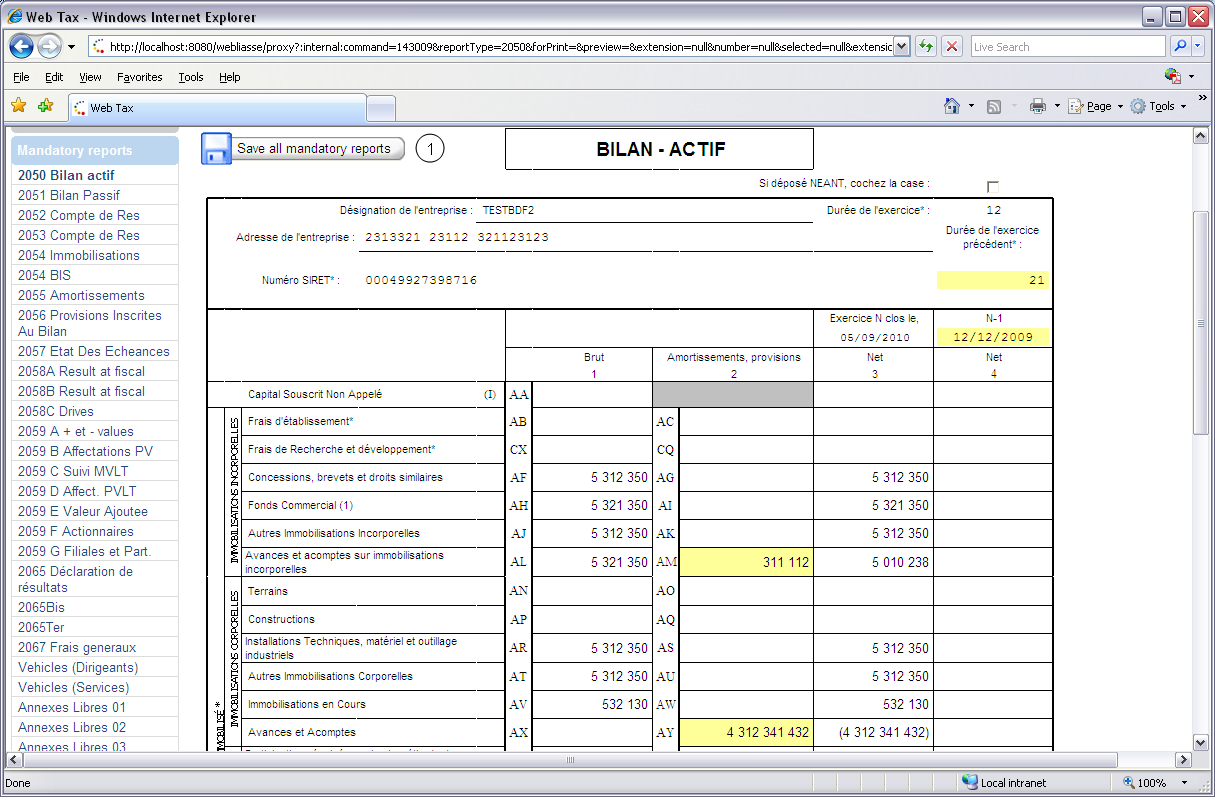
\includegraphics[width=0.9\textwidth]{pics/src_reportnice}
  \end{center}
\end{frame}


\section{Тестирование}
\subsection{Модульные тесты}
\begin{frame}
  \frametitle{Модульные тесты}
  В целях тестирования кода и контроля качества во время разработки были реализованы модульные тесты.
  Результат выполнения:
  \begin{center}
    \small {
      \rowcolors{1}{RoyalBlue!20}{RolalBlue!5}
      \begin{tabular}{|m{4cm}|m{2cm}|m{2cm}|} \hline
        Класс & Кол-во тестов & Успешные тесты \\ \hline
        ReportFactoryImplTest & 1 & 100\% \\ \hline
        ReportManagerTest & 3 & 100\% \\ \hline
        ReportCrossInterpreterTest & 1 & 100\% \\ \hline
        ReportInterpreterTest & 1 & 100\% \\ \hline
        XMLReportLoaderTest & 1 & 100\% \\ \hline
        XMLCellLoaderTest & 2 & 100\% \\ \hline
        XMLFileReaderTest & 3 & 100\% \\ \hline
        AccountsInterpreterTest & 1 & 100\% \\ \hline
        ReflectionAssemblerTest & 1 & 100\% \\ \hline
        ExpressionParserTest & 2 & 100\% \\ \hline
      \end{tabular}
    }
  \end{center}
\end{frame}

\section{Заключение}
\begin{frame}
  \frametitle{Заключение}
  Для выполнения дипломного проекта были решены следующие задачи:
  \begin{itemize}
    \item Анализ предметной области
    \item Проектирование системы
    \item Реализация системы
    \item Тестирование системы
    \item Выделение мер, обеспечивающих комфортные условия труда разработчикам систем документооборота
    \item Произведено технико-экономическое обснование эффективности внедрения программного продукта
  \end{itemize}
\end{frame}


\end{document}
